\begin{surferPage}{Chmutov의 $8$차식}
   우리의 눈을 사로잡는 Chmutov의 $8$차식 $\text{Chm}_{d}, \ d=8$ 의 특징은 대칭성입니다. 
   이 대칭성은 방정식을 통해서도 짐작할 수 있습니다.
    \[\text{Chm}_{d}\colon T_d(x) + T_d(y) + T_d(z) + 1 = 0,\]
    여기서 $T_d$는 잘 알려진 체비셰프 다항식입니다(아래 왼쪽). 곡선 $T_8(x)+T_8(y)=0$ 는 오른쪽에 그려져 있습니다. 
    
     \begin{center}
      \begin{tabular}{c@{\quad}c}
        \begin{tabular}{c}
          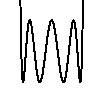
\includegraphics[height=1.75cm]{./../../common/images/Tcheb_008.pdf}
        \end{tabular}    
        &
        \begin{tabular}{c}
          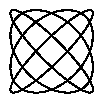
\includegraphics[height=1.75cm]{./../../common/images/Tcheb_2d_008.pdf}
        \end{tabular}    
      \end{tabular}
    \end{center}
    \vspace{-0.3cm}
    앞의 두 그림을 통해 오른쪽 곡면을 얻는 과정은 그리 복잡하지 않습니다. 


이 방정식은 80년대 S.V.\ Chmutov에 의해 발견되었습니다. 당시 이러한 형태의 방정식은 대부분의 차수 $d$에 대하여 세계기록을 가지고 있었습니다. 90년대에 Chmutov는 자신의 기록을 더욱 발전시켰고 2005년에 S.~Breske, O.~Labs 그리고 D.~van~Straten는 이를 이용하여 실수 특이점만 갖는 실수 곡면들을 찾아냈습니다.
\end{surferPage}
